\section{Bolting ``Kill'em All''}

\margininbox{Kill'em All}{
     \begin{itemize}
    \item Iztok Možir
    \item Richard Venn
    \end{itemize}}{\explo}

During the ever long breakfast in the \passage{Bivi}, Rick was asking who wants to
go with him to \passage{Captain Kangaroo}. Nobody volunteered immediately. Tetley
said he can go, but only to \passage{Bonus chamber} and then pointed to me and
said, ``Izi, you should go!'' I agreed and soon we were packing all the
necessary equipment.

This was my first time in \passage{Vrtnarija} and at the beginning was nothing to
serious, lovely pitches, couple of squeezes and soon we were on top of
\passage{Pico}. Rick warned me to use the red rope, which is going right into the
\passage{Captain Kangaroo}. Before we enter the Captain Rick said, ``So, this is
it! Now fun begins!'' We all smoked one and off we go. Tetley turned
back at \passage{Bonus chamber}. Rick knew the way on so he was the leader. We
soon arrived to \passage{Mudslump} with few very tight and tricky squeezes.

\begin{marginfigure}
\checkoddpage \ifoddpage \forcerectofloat \else \forceversofloat \fi
\centering
 \frame{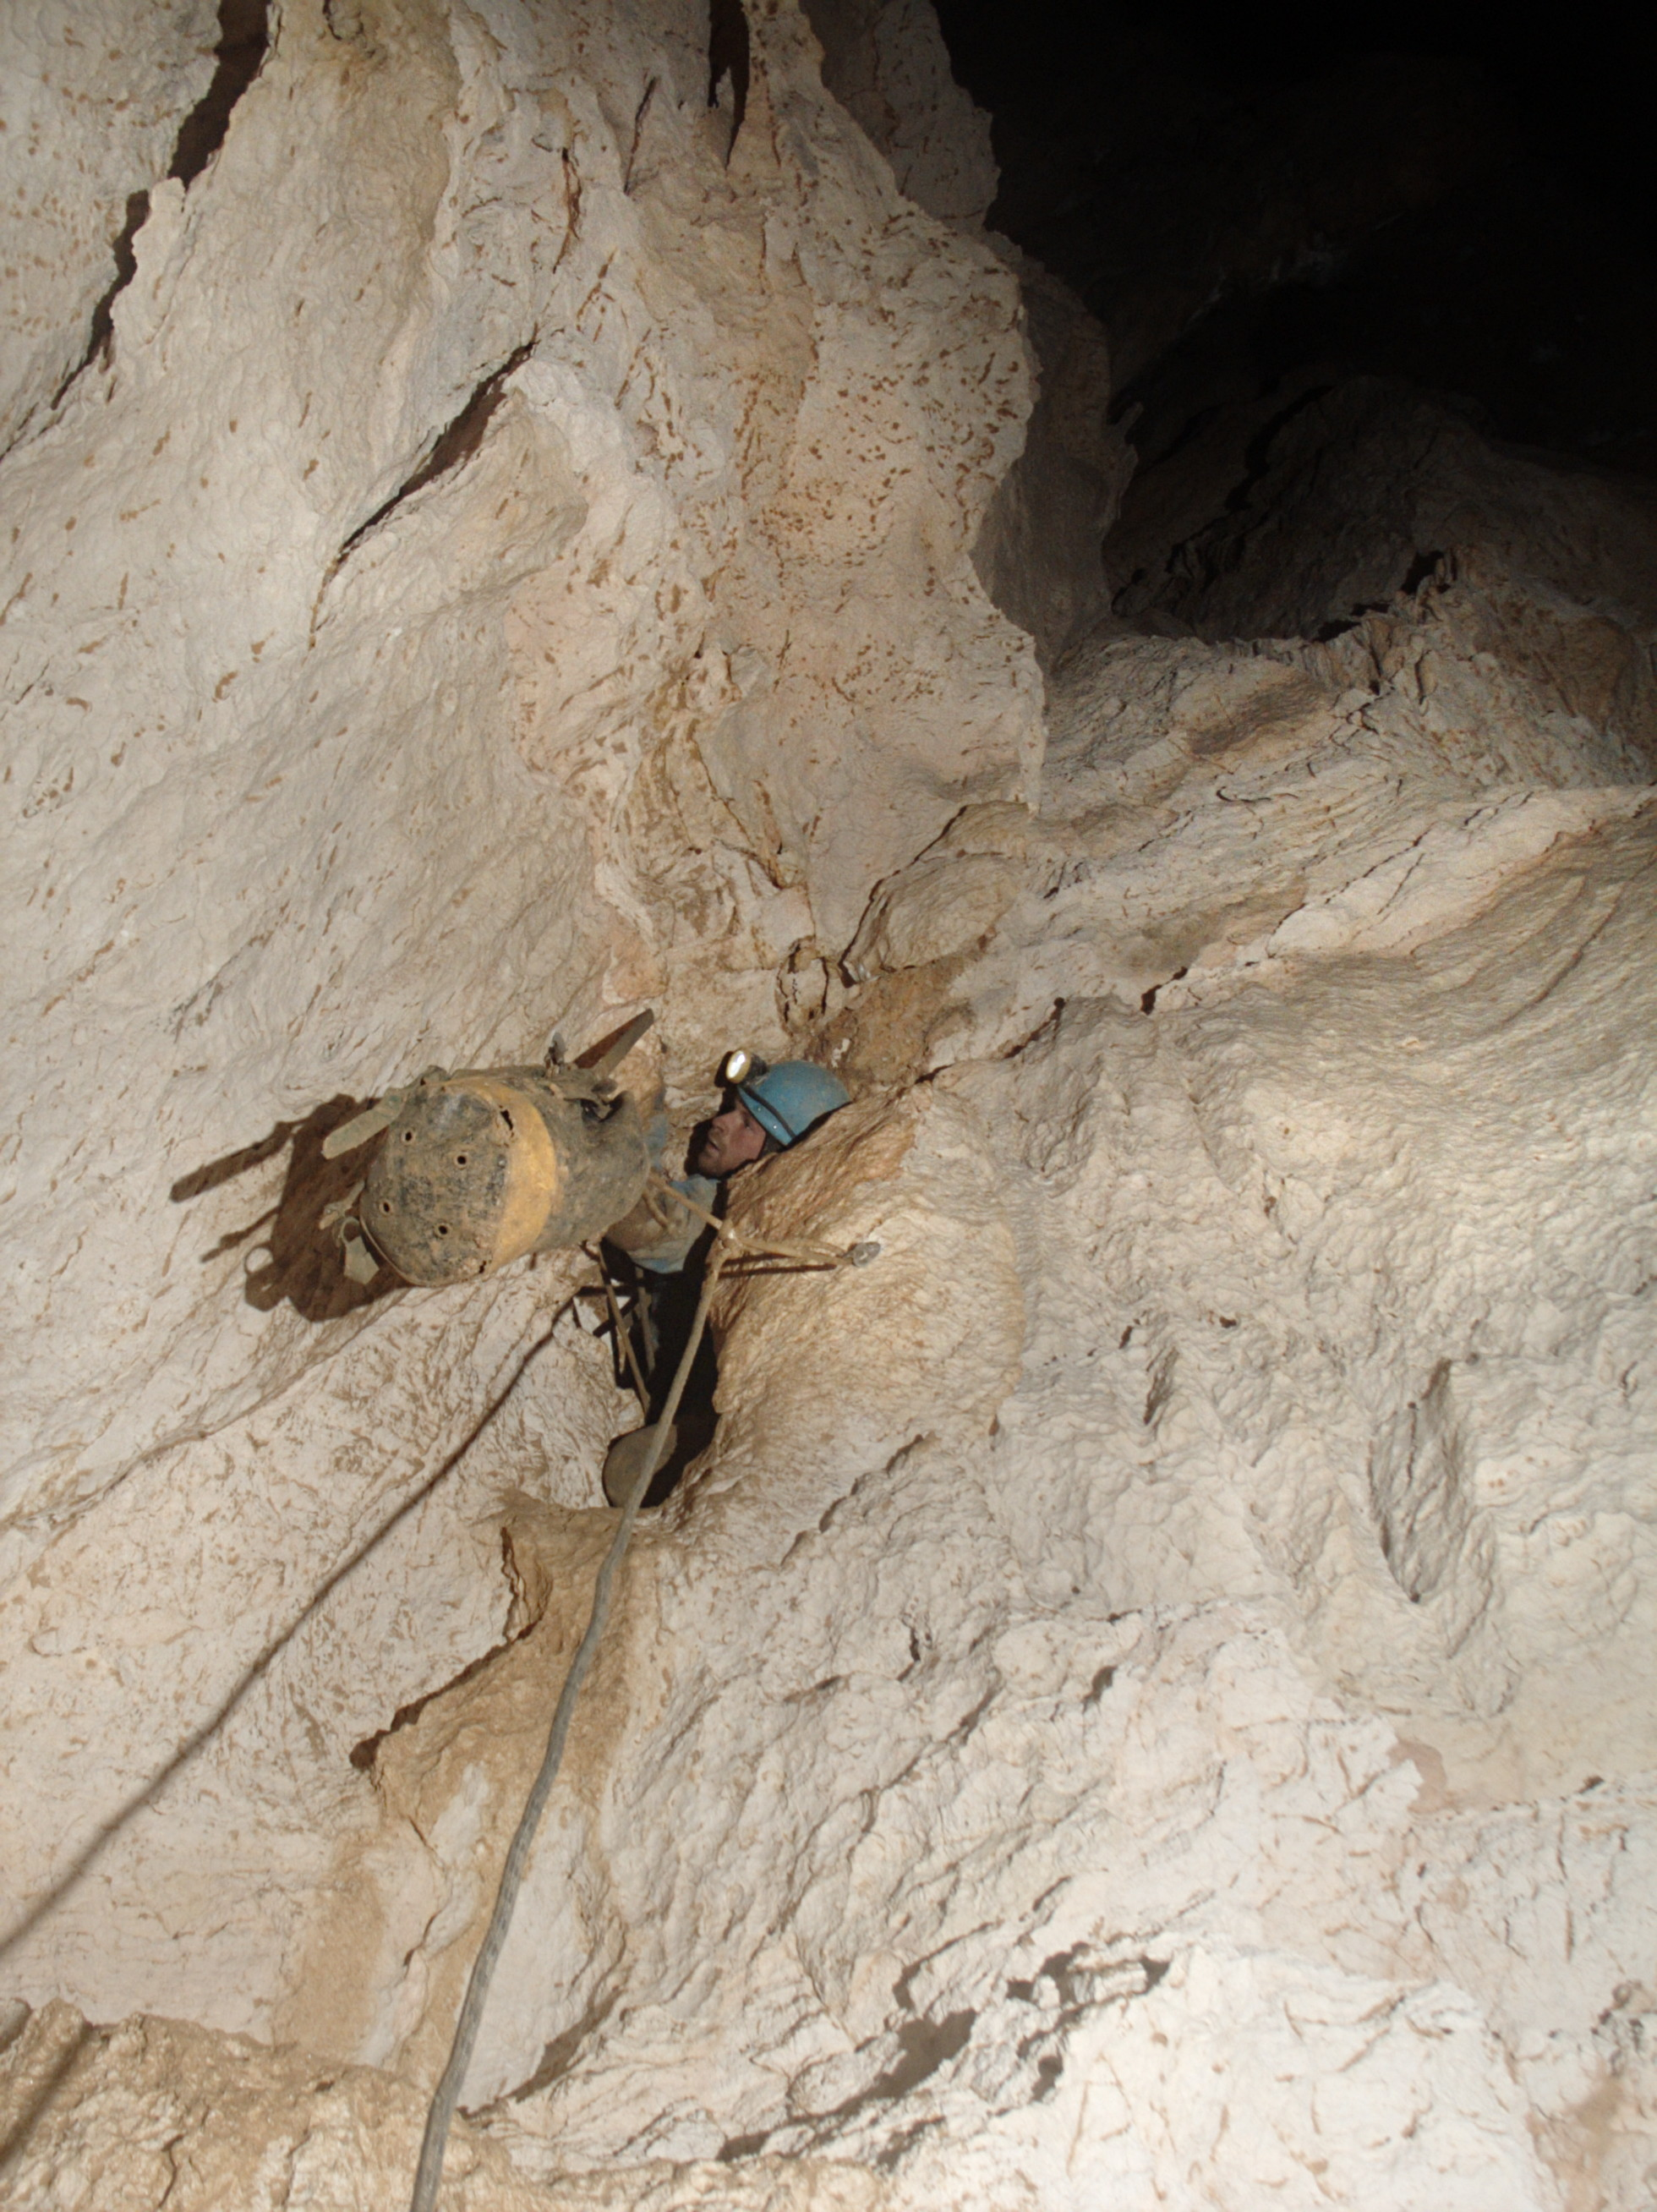
\includegraphics[width=\linewidth]{2007/kill_em_all/2009-08-06-15.01.44 - Jarvist Frost - Canon Powershot G5 - killem all - mike at pitch head struggling with bag--orig.jpg}} 
 \caption{Mike Foley struggles with a tackle bag at the pitch head of \protect\passage{Kill'em All} in 2009 while Jarvist Frost waits on the rope below. \pic{Jarvist Frost}}
 \label{Kill em All Mike}
\end{marginfigure}

Once through, we free climbed couple of small pitches and arrived to a
small chamber. The way on was through a squeeze which led to a top of
the pitch. It was very little space here, not even enough to do the
bolting properly. After couple of minutes of thinking and couple of
cigarettes we had a plan. One of us would go on the rope, while the
other one will attach the rope to his croll, get stuck in the squeeze
and hold the other one until bolting finished. Rick was brave enough to
trust me, so he did the bolting. During the bolting I smoked a lot and
we chatted about the music. We both knew the first Metallica album and
so we decide to name this pitch \passage{Kill'em All}. The way down was no
problem and while descending we spotted lots of windows. On the bottom
we cut the rope, leave the rest there and started surveying on way out.
Rick went up first and it took him a while to get the rope free. 

Finally, I went up and soon realised what took Rick so long. When we were bolting
we were not paying attention on how low the bolts are. Now \bignote{the only way
to go off the rope was to undo your croll and step into the Y hang and
somehow throw yourself into the pitch head squeeze}. Overall, a very
enjoyable caving journey with Rick. Once in the \passage{Bivi}, we entered the
data into Survex and we realised we were very close to the bottom of
\passage{Silos} (\passage{M2}).

\name{Iztok Možir}



